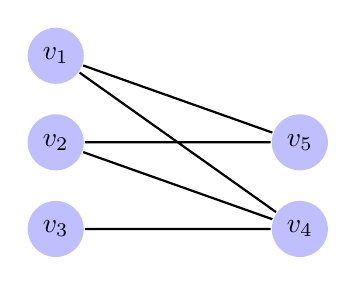
\begin{tikzpicture}[auto, thick, node distance=1.1cm,every node/.style={circle,fill=blue!25}]
	\node (p0) {$v_1$};
	\node (p1) [below of=p0] {$v_2$};
	\node (p2) [below of=p1] {$v_3$};
	\node (p3) [right of=p2,xshift=2cm] {$v_4$};
	\node (p4) [above of=p3] {$v_5$};
	
	\draw
	(p0) -- (p3)
	(p0) -- (p4)
	(p1) -- (p3)
	(p1) -- (p4)
	(p2) -- (p3);
\end{tikzpicture}
